\subsection{Number of Contacts}
\label{subsec:data_number_of_contacts}

We calibrate the parameters for the predicted numbers of contacts from contact diaries
of over 2000 individuals from Germany, Belgium, the Netherlands and Luxembourg
\citep{Mossong2008}. Each contact diary contains all contacts an individual had
throughout one day, including information on the other person (such as age and gender)
and information on the contact. Importantly, for each contact individuals entered of
which type the contact (school, leisure, work etc.) was and how frequent the contact
with the other person is.

Simplifying the number of contacts, we arrive at the following distributions of the
numbers of contacts by contact type.

\begin{figure}
    \centering
    % other contacts
    \begin{subfigure}[b]{0.3\textwidth}
        \centering
        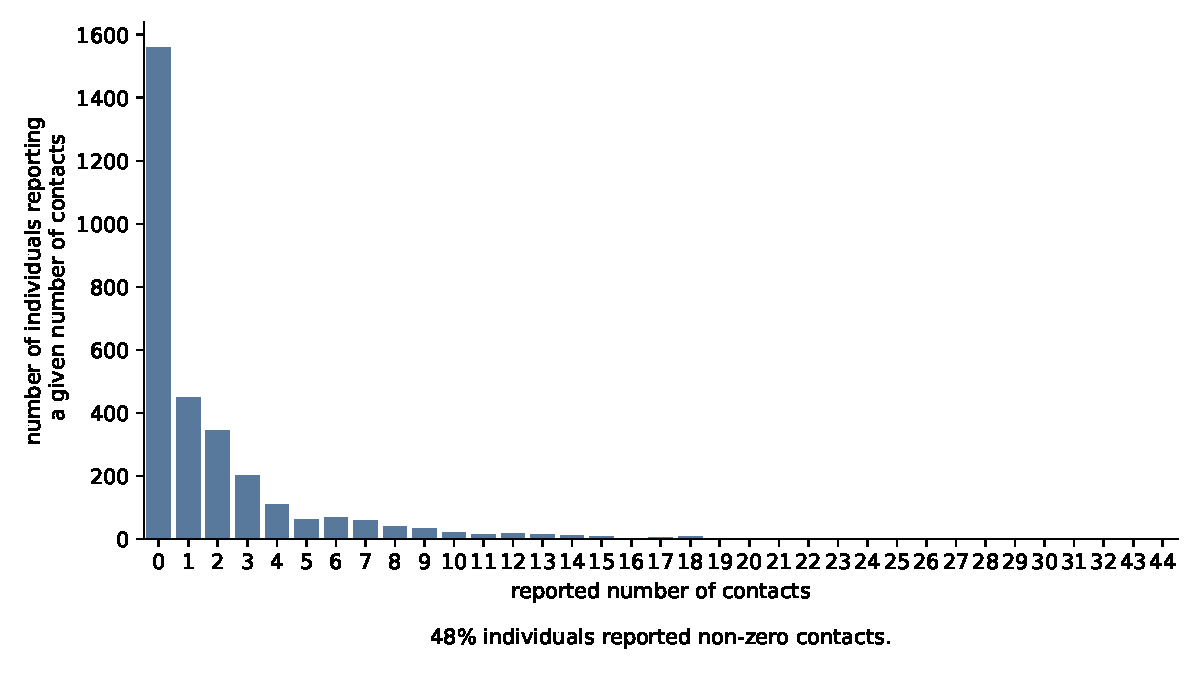
\includegraphics[width=\textwidth]{figures/results/figures/data/distributions_of_the_number_of_contacts/other_non_recurrent}
        \caption{Number of Non Recurrent Other Contacts}
        \label{n_contacts_other_non_recurrent}
    \end{subfigure}
    \hfill
    \begin{subfigure}[b]{0.3\textwidth}
        \centering
        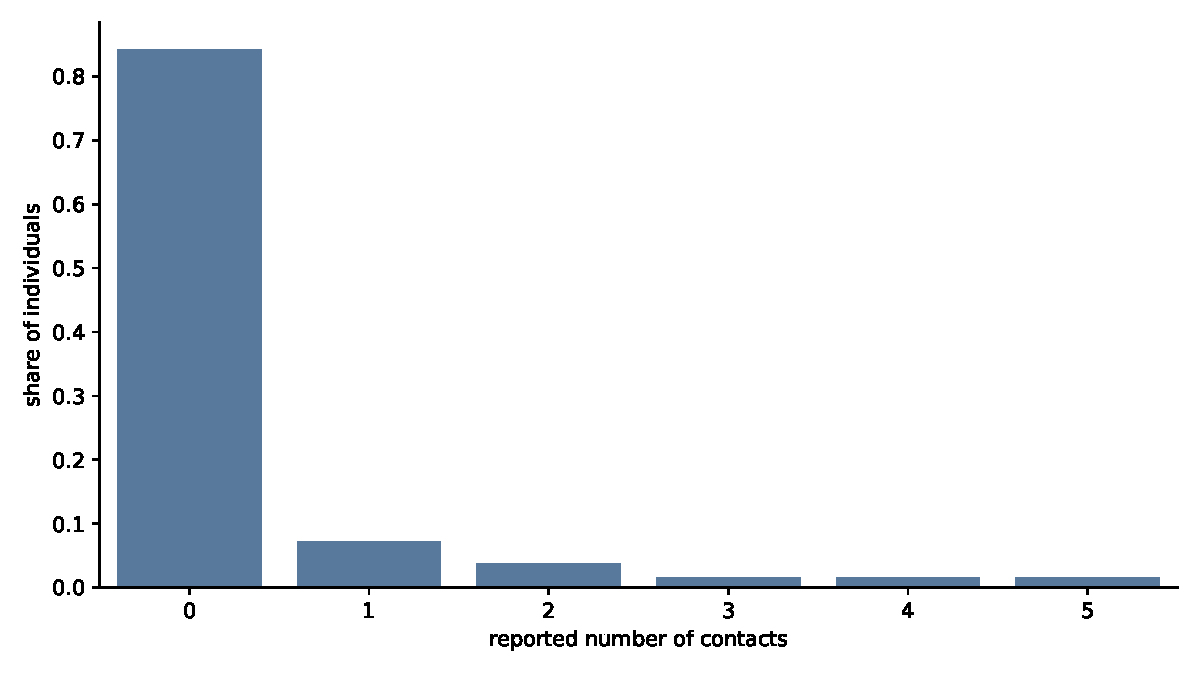
\includegraphics[width=\textwidth]{figures/results/figures/data/distributions_of_the_number_of_contacts/other_recurrent_daily}
        \caption{Number of Daily Recurrent Other Contacts}
        \label{n_contacts_other_daily_recurrent}
    \end{subfigure}
    \hfill
    \begin{subfigure}[b]{0.3\textwidth}
        \centering
        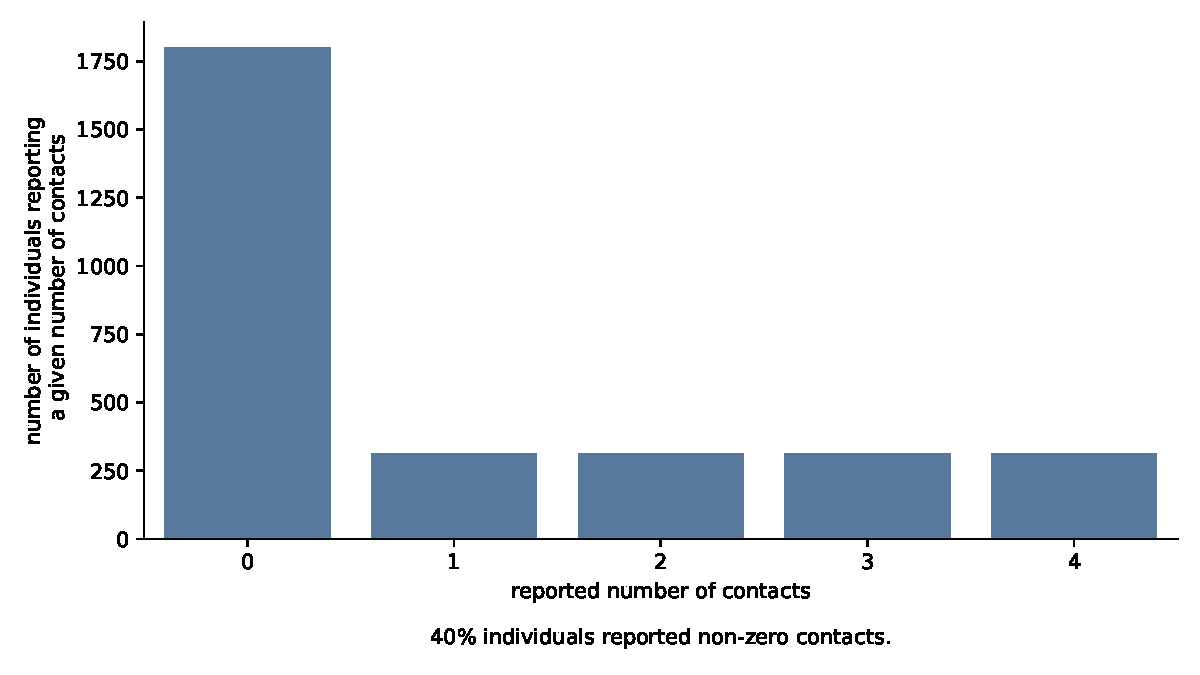
\includegraphics[width=\textwidth]{figures/results/figures/data/distributions_of_the_number_of_contacts/other_recurrent_weekly}
        \caption{Number of Weekly Recurrent Other Contacts}
        \label{n_contacts_other_weekly_recurrent}
    \end{subfigure}

    \vskip3ex

    % work contacts
    \begin{subfigure}[b]{0.3\textwidth}
        \centering
        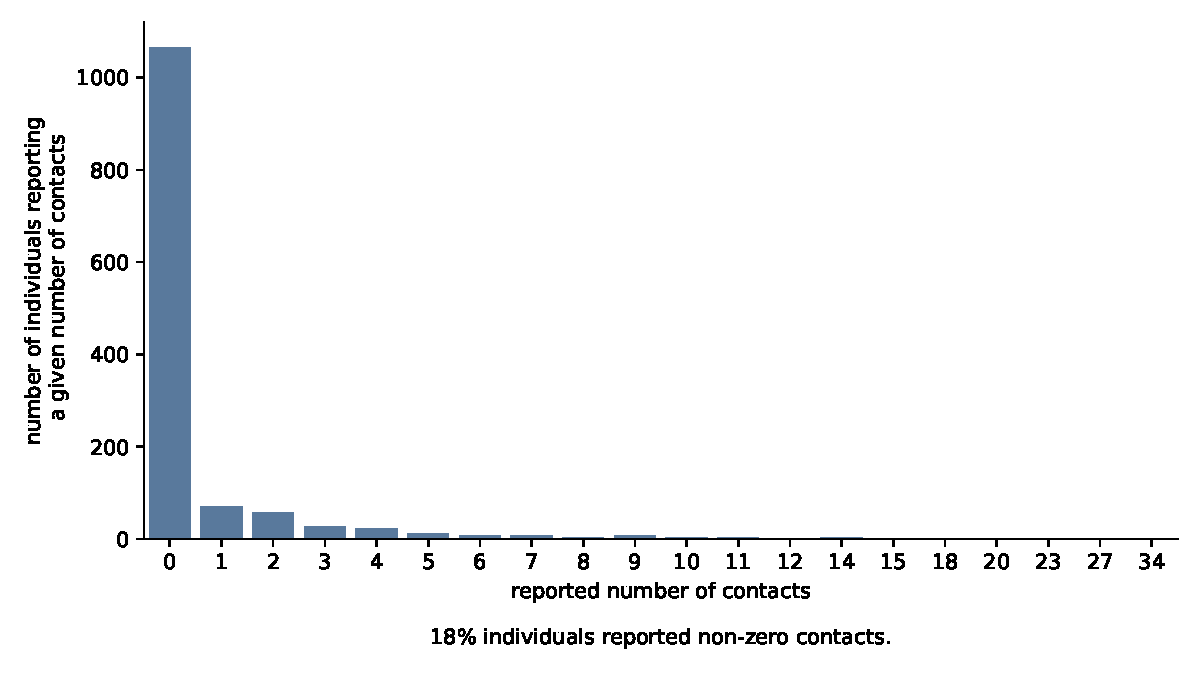
\includegraphics[width=\textwidth]{figures/results/figures/data/distributions_of_the_number_of_contacts/work_non_recurrent}
        \caption{Number of Non Recurrent Work Contacts}
        \label{n_contacts_work_non_recurrent}
    \end{subfigure}
    \hfill
    \begin{subfigure}[b]{0.3\textwidth}
        \centering
        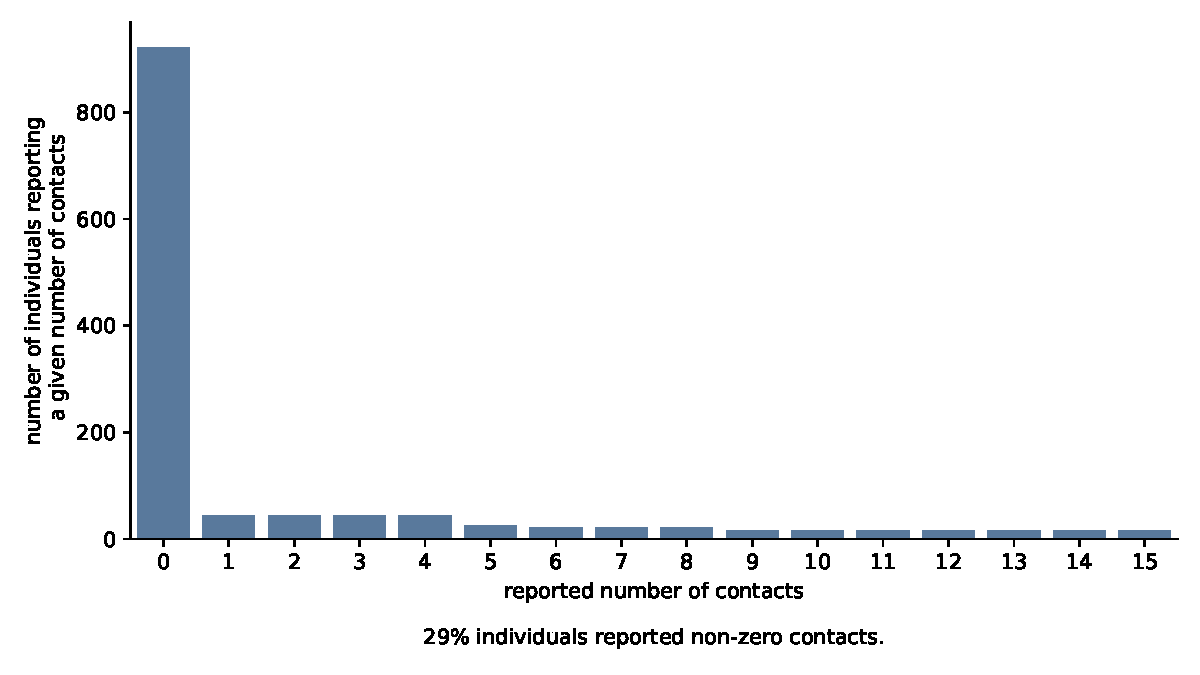
\includegraphics[width=\textwidth]{figures/results/figures/data/distributions_of_the_number_of_contacts/work_recurrent_daily}
        \caption{Number of Daily Recurrent Work Contacts}
        \label{n_contacts_work_daily_recurrent}
    \end{subfigure}
    \hfill
    \begin{subfigure}[b]{0.3\textwidth}
        \centering
        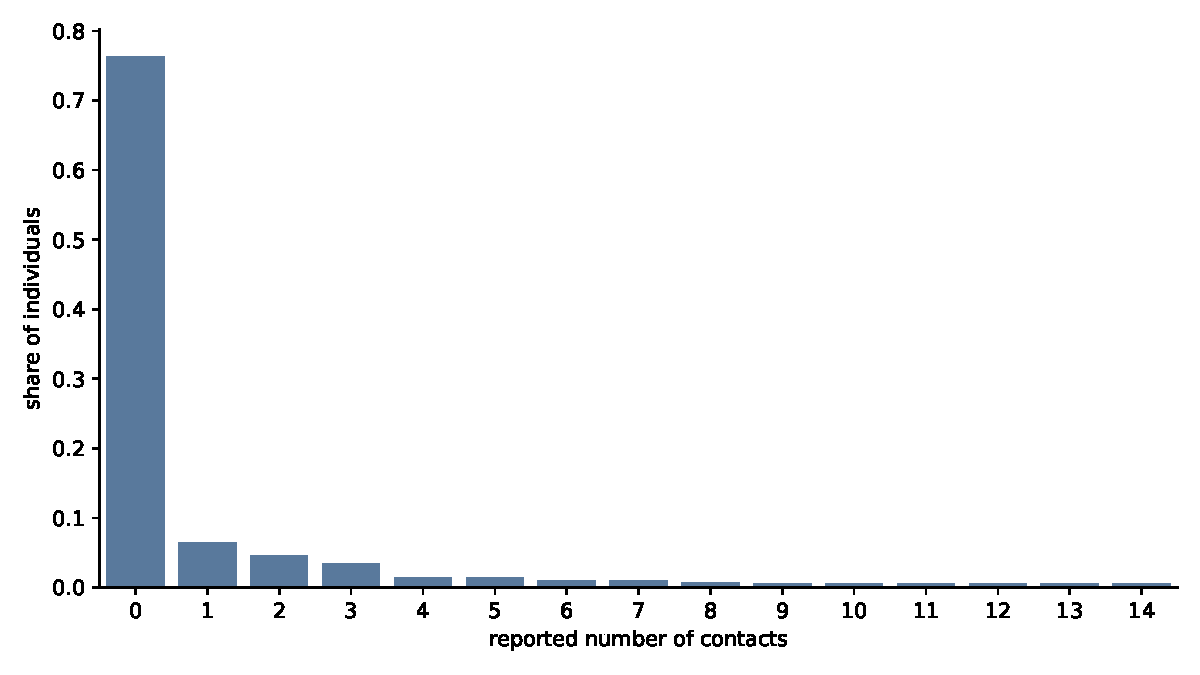
\includegraphics[width=\textwidth]{figures/results/figures/data/distributions_of_the_number_of_contacts/work_recurrent_weekly}
        \caption{Number of Weekly Recurrent Work Contacts}
        \label{n_contacts_work_weekly_recurrent}
    \end{subfigure}
    \vskip3ex

    \caption{Number of Contacts of the Different Contact Types}
    \label{fig:n_contacts_other}
    \floatfoot{\noindent
        \textit{Note:} The upper row shows the distribution of the number of other
        contacts individuals report. Other contacts include all contacts that are not
        household members, school contacts or work contacts, for example leisure
        contacts. The planned number of contacts is reduced by policies, seasonality and
        individual responses to events such as receiving a positive rapid test to the
        number of actual contacts with transmission potential.
        % non recurrent
        In the model it is sampled every day which of the numbers of non recurrent
        contacts a person is planned to have. Note that the contact diaries include such
        high values that super spreading events are well possible in our model through
        non recurrent other models. We assume that individuals in households with
        children or teachers or retired individuals have additional non recurrent
        contacts during school vacations to cover things like family visits or travel
        during vacations. We estimate this to be on average 0.5 additional contacts per
        vacation day.
        % daily and weekly
        For the recurrent other contacts, individuals are assigned to groups that are
        time constant and that meet daily or weekly. The share of individuals who attend
        in a way that has transmission potential is reduced by policies, seasonality and
        individual responses to events such as receiving a positive rapid test. For
        weekly contacts, individuals are assigned to up to four groups that are time
        constant and that meet weekly. The day on which meetings take place varies
        between groups but stays the same for each group.
        % work contacts
        The lower row shows the distribution of the different types of work contacts.
        Work contacts only take place between working individuals.
        % non recurrent
        In the model it is sampled every day which number of non recurrent work contacts
        a working person is planned to have. Note that the contact diaries include such
        high values that super spreading events are well possible in our model. The
        planned number of contacts is reduced by policies, seasonality and individual
        responses to events such as receiving a positive rapid test to the number of
        actual contacts with transmission potential.
        % daily
        Working individuals are assigned to groups that are time constant and that meet
        daily to match the given distribution of daily work contacts. This contact type
        covers contacts such as colleagues with which one shares an office space. The
        share of individuals who attend in a way that has transmission potential is
        reduced by policies (such as a work from home mandate), seasonality and
        individual responses to events such as receiving a positive rapid test.
        % weekly
        Working individuals are assigned to up to 14 groups that are time constant and
        meet weekly. Groups are scheduled to meet on separate days of the work week.
        These contact models cover weekly team meetings etc. The share of individuals
        that attend in a way that has transmission potential is reduced by policies,
        seasonality and individual responses to events such as receiving a positive rapid
        test.}
\end{figure}


An exception where we do not rely on the data by \cite{Mossong2008} are the household
contacts. Since household are included in the the German microcensus
\citep{FDSAeDBUDL2018} on which we build our synthetic population we simply assume for
the household contact model that individuals meet all other household members every day.


\begin{figure}
    \centering
    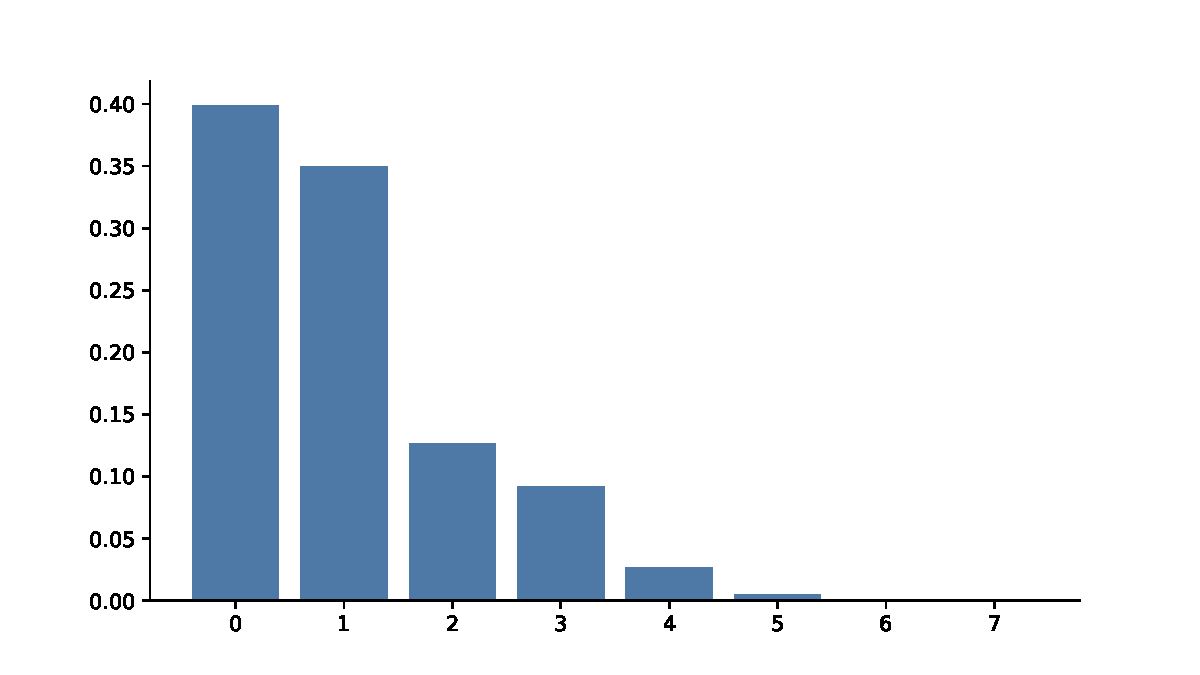
\includegraphics[width=0.5\textwidth]{figures/results/figures/data/distributions_of_the_number_of_contacts/household}
    \caption{Number of Household Contacts}
    \label{n_contacts_hh}
    \floatfoot{\noindent
        \textit{Note:} Every individual meets all other household members every day. The
        German microcensus sampled full households such that our synthetic population
        automatically fits population characteristics such as size and age distribution.}
\end{figure}

\FloatBarrier